\documentclass[tikz, border=10pt]{standalone}
\usepackage{tikz}
\usepackage{amsmath}
\usetikzlibrary{arrows.meta, decorations.pathmorphing}
\usepackage{xcolor}
\begin{document}
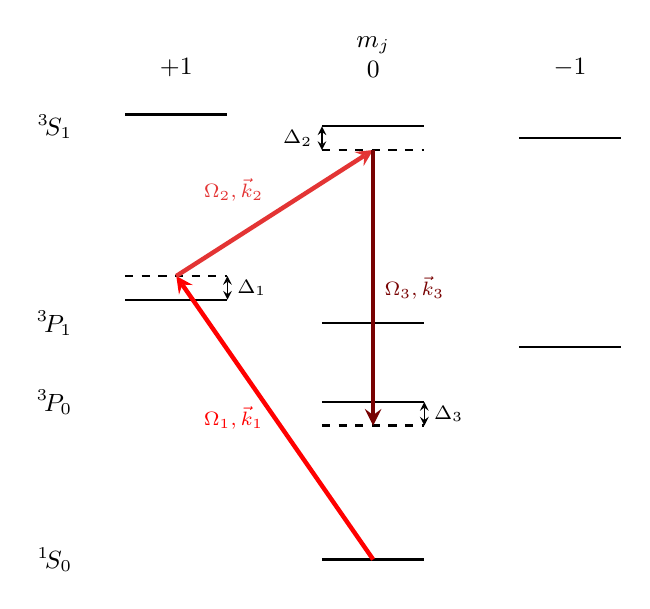
\begin{tikzpicture}

% -------------------------------------------------------
% Layout parameters
% -------------------------------------------------------
\def\lw{0.65}     % half-length of sublevel lines
\def\dz{0.3}     % Zeeman sublevel spacing (schematic)
\def\offset{2.5}
\def\detune{0.3}
\def\lboff{-3.7}
\def\mjoff{0.5}

% X centers for each level/manifold
\def\xGnd{0}
\def\xPo{0}
\def\xPz{0}
\def\xSo{0}

% Y positions
\def\yGnd{-0.5}
\def\yPz{2.5}     % 3P0 (~14504 cm^{-1})
\def\yPo{1.5}     % 3P1 center (~14836 cm^{-1})
\def\ySo{5}     % 3S1 center (~29038 cm^{-1})

% colors
\definecolor{c689}{HTML}{ff0000}
\definecolor{c688}{HTML}{E33434}
\definecolor{c679}{HTML}{780202}

\tikzstyle{arrow} = [ultra thick,->,>=stealth];



%%%%%% DRAW LEVELS
% 1S0
\draw[thick] (\xGnd-\lw, \yGnd) -- (\xGnd+\lw, \yGnd);
\node[left, font=\small] at (\xGnd + \lboff, \yGnd) {${}^1\!S_0$};


%3P0
\draw[thick] (\xPo-\lw, \yPo) -- (\xPo+\lw, \yPo);
\draw[thick, dashed] (\xPo-\lw, \yPo-\detune) -- (\xPo+\lw, \yPo-\detune); % detuning
\draw[<->, >=stealth, font=\scriptsize] (\xPo +\lw, \yPo - \detune) -- (\xPo +\lw , \yPo ) node[midway, right] {$\Delta_3$};

\node[left, font=\small] at (\xPo + \lboff, \yPo) {${}^3\!P_0$};


%3P1 + SUBLEVELS
\draw[thick] (\xPz-\lw - \offset, \yPz+\dz) -- (\xPz+\lw - \offset, \yPz+\dz); %MJ=+1
\draw[thick] (\xPz-\lw, \yPz)     -- (\xPz+\lw, \yPz);%MJ=0
\draw[thick] (\xPz-\lw + \offset, \yPz-\dz) -- (\xPz+\lw+\offset, \yPz-\dz);%MJ=-1
\draw[thick, dashed] (\xPz-\lw - \offset, \yPz+\dz+\detune) -- (\xPz+\lw - \offset, \yPz+\dz+\detune); % detuning
\draw[ <->, >=stealth, font=\scriptsize] (\xPz - \offset + \lw, \yPz+\dz ) -- (\xPz+\lw - \offset, \yPz+\dz + \detune) node[midway, right] {$\Delta_1$};
\node[left, font=\small] at (\xPz + \lboff, \yPz) {${}^3\!P_1$};

%3S1 + SUBLEVELS
\draw[thick] (\xSo-\lw + \offset, \ySo-\dz/2) -- (\xSo+\lw + \offset, \ySo-\dz/2);%MJ=+1
\draw[thick] (\xSo-\lw, \ySo)     -- (\xSo+\lw, \ySo);%MJ=0
\draw[thick] (\xSo-\lw - \offset, \ySo+\dz/2) -- (\xSo+\lw - \offset, \ySo+\dz/2);%MJ=-1
\draw[thick, dashed] (\xSo-\lw , \ySo-\detune) -- (\xSo+\lw, \ySo-\detune); % detuning
\draw[ <->, >=stealth, font=\scriptsize] (\xSo  - \lw, \ySo) -- (\xSo - \lw, \ySo - \dz) node[midway, left] {$\Delta_2$};

\node[left, font=\small] at (\xSo + \lboff, \ySo) {${}^3\!S_1$};


%%%%%% DRAW TRANSITIONS
\draw[arrow, c689, font=\scriptsize] (\xGnd, \yGnd) -> (\xPz - \offset, \yPz + \dz + \detune) node[midway, left] {$\Omega_{1}, \vec{k}_{1}$};
\draw[arrow, c688, font=\scriptsize] (\xPz - \offset, \yPz + \dz + \detune) -> (\xSo , \ySo-\detune) node[midway, above left] {$\Omega_{2}, \vec{k}_{2}$};
\draw[arrow, c679, font=\scriptsize]  (\xSo , \ySo-\detune) -> (\xPo , \yPo - \detune) node[midway, right] {$\Omega_{3}, \vec{k}_{3}$};

%%% ZEEMAN LABELS
\node[left, font=\small] at (\xGnd - \offset, \ySo + \mjoff) [above] {$+1$};
\node[left, font=\small] at (\xGnd, \ySo + \mjoff) [above] {$0$};
\node[left, font=\small] at (\xGnd, \ySo + \mjoff + 0.3) [above] {$m_j$};
\node[left, font=\small] at (\xGnd + \offset, \ySo + \mjoff) [above] {$-1$};



% \draw[draw=black] (\xGnd - \offset - \lw -0.2, \yGnd - 0.2) rectangle ++(2*\offset + 2*\lw + 0.4, \ySo + 1.2);



\end{tikzpicture}
\end{document}
